%	\item Begrundelse baseret på antal op-amp / orden (6/8)
%	\item Kort teoretisk gennemgang af den valgte topologi
%	\item Beregninger og dimensionering af 6. ordens chebycheb filtre
%	\item Implementeringsvalg og design af hardware/schematics
%\end{itemize}


\section{Analoge filtres rolle ved digital signalbehandling}\label{sec:filter_intro}
\note{Kort teoretisk intro til hvorfor filtre skal anvendes til sampling}
\note{Båndbrede begrænsning}
\note{Shannons sampling theorem}
\note{Generel intro til audio signaler}
\note{begrundelse for orden af filter i intro}

\section{Analyse af filter typer}\label{sec:filter_analyse}
\note{Gennem gang af de filter topologier der har været i betragtning som en mulig løsning.}
For at kunne finde frem til et passende lavpasfilter som antialiasing filter, bliver 4 tilter typer sammenlignet - Butterworth, Chebyshev type I og II samt Bessel (Thomson).
Hver af disse filtre har en tilhørende amplitudekarakteristik der beskrives med følgende overføringsfunktion\cite{anfilter}.

\begin{align} 
H_{butterworth}(j\omega_n) &= \frac{1}{\sqrt{1 + \omega_n^{2n}}} \label{eq:H_butt} \\
H_{bessel} (j\omega_n) &= \frac{H}{a_0 + \omega^2 + ja_1\omega_n} \label{eq:H_bes}\\
H_{chebychevI}(j\omega_n) &= \frac{1}{\sqrt{1 + \epsilon^2 C_n^2(\omega_n)}} \label{eq:H_cheb1} \\
H_{chebychevII}(j\omega_n) &= \frac{1}{\sqrt{1 + \frac{1}{\epsilon^2 C_n^2(\omega_n)}}} \label{eq:H_cheb2} \\
C_n(\omega_n) &=  
\begin{matrix}
	\cos(n\arccos(\omega_n)) & 0 \le \omega_n \le 1 \\  \cosh(n \arccosh(\omega_n)) & 1 \le \omega_n 
\end{matrix} \label{eq:chev_cn_funk}
\end{align}

I ligning (\ref{eq:chev_cn_funk}) fremgår den indre funktion $C_n(\omega_n)$ som bruges i Chebychev I og II i ligening (\ref{eq:H_cheb1}) og (\ref{eq:H_cheb2}).

Figur \ref{fig:filter_typer} viser en samlet fremstilling af amplitude karakteristikken $H(j\omega_n)$ og gruppeløbstiden $D(\omega_n)$ for de fire filtertyper.

\begin{figure}[h!]
	\centering
	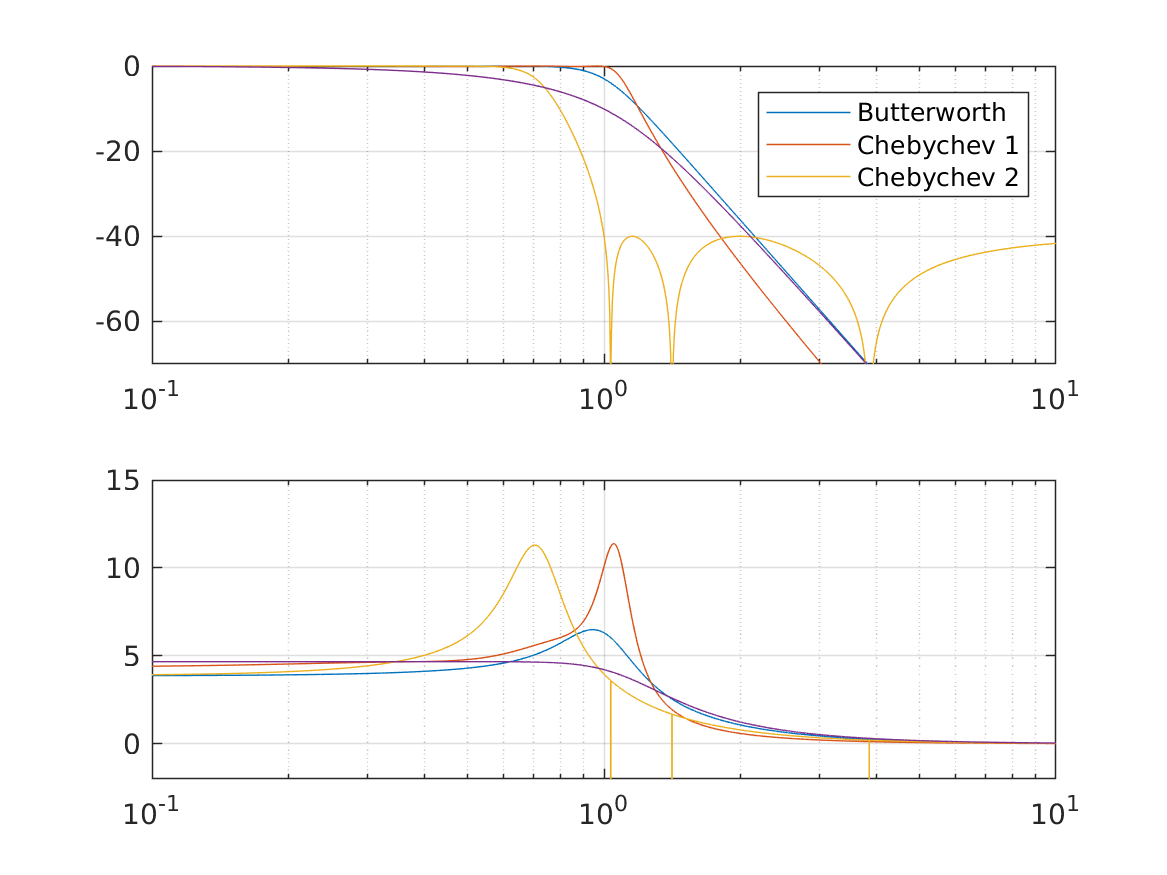
\includegraphics[width=1\textwidth]{matlab/filter_compare.png}
	\caption{Normeret 6.ordens filter karakteristik (øverst) og guppeløbstid (nederst) for filtertyperne Butterworth, Chebychev Type I ($0,1 \si{\decibel}$ rippel) \& Type II ($-40 \si{\decibel}$ stopbånds rippel) og Bessel.}
	\label{fig:filter_typer}
\end{figure}

Det ønskede filter skal have en rimelig flad karakteristisk i pasbåndet og en stejl overgang til stopbåndet.
Således kan lydsignalets amplitude holdes konstant i hele det ønskede frekvensområde da uønsket dæmpning/forstærkning af lydsignalet kan medfører hørbare ændringer af lydbilledet, på samme måde som en equalizer påvirker et lydsignal. 

Ligeledes ønskes en rimelig konstant gruppeløbetid. 
Gruppeløbetiden, der er defineret i ligning (\ref{eq:groupdelay_def})\cite{anfilter}, er et udtryk for hvor stor tidsforsinkelsen på signal som funktion af frekvensen er.

\begin{align}
	D(\omega) \stackrel{def}{=} - \dfrac{d(arg(N(\omega)))}{d\omega}\label{eq:groupdelay_def}
\end{align}

Hvis signal forsinkelsen bliver for stor i et givet frekvensområde, vil der fremstå en hørbar ændring af lydbilledet.
Dette fenomen er dog ret subjektivt og der findes mange meninger om hvilke tærskelværdier der kan accepteres.
Ud fra en lettere gennemgang inden for området, er antages en acceptabel relativ tidsforsinkelse på $D_{rel}(\omega) < -10 \si{\milli\second}$ til projektet.   

\subsection{Valg af filter topologi}
Hvis man som udgangspunkt kun fokusere på filtrenes gruppeløbstid, ville man skulle vælge et Bessel filter.
Bessel filteret, det er designet som et filter med maksimal fald fase, har dog langt fra den ønskede dæmpning i overgangsbåndet.
Det vælges at anvende et Chebychev type I filter, der viser sig at have den bedste dæmpning i overgangsbåndet.
Det høje udsving på gruppeløbetiden for denne filtertype, som det fremgår i figur \ref{fig:filter_typer}, vil på det denomaliserede filter ligger indenfor, de i projektet, acceptable værdier. 
\\
I figur \ref{fig:filter_cheb1_denorm} ses den denormaliserede filterkarakteristik for det valgte filter med en pasbåndsrippel på $0,1 \si{\decibel}$ og en knækfrekvens på $f_c = 18 \si{\kilo\hertz}$. 

\begin{figure}[h!]
	\centering
	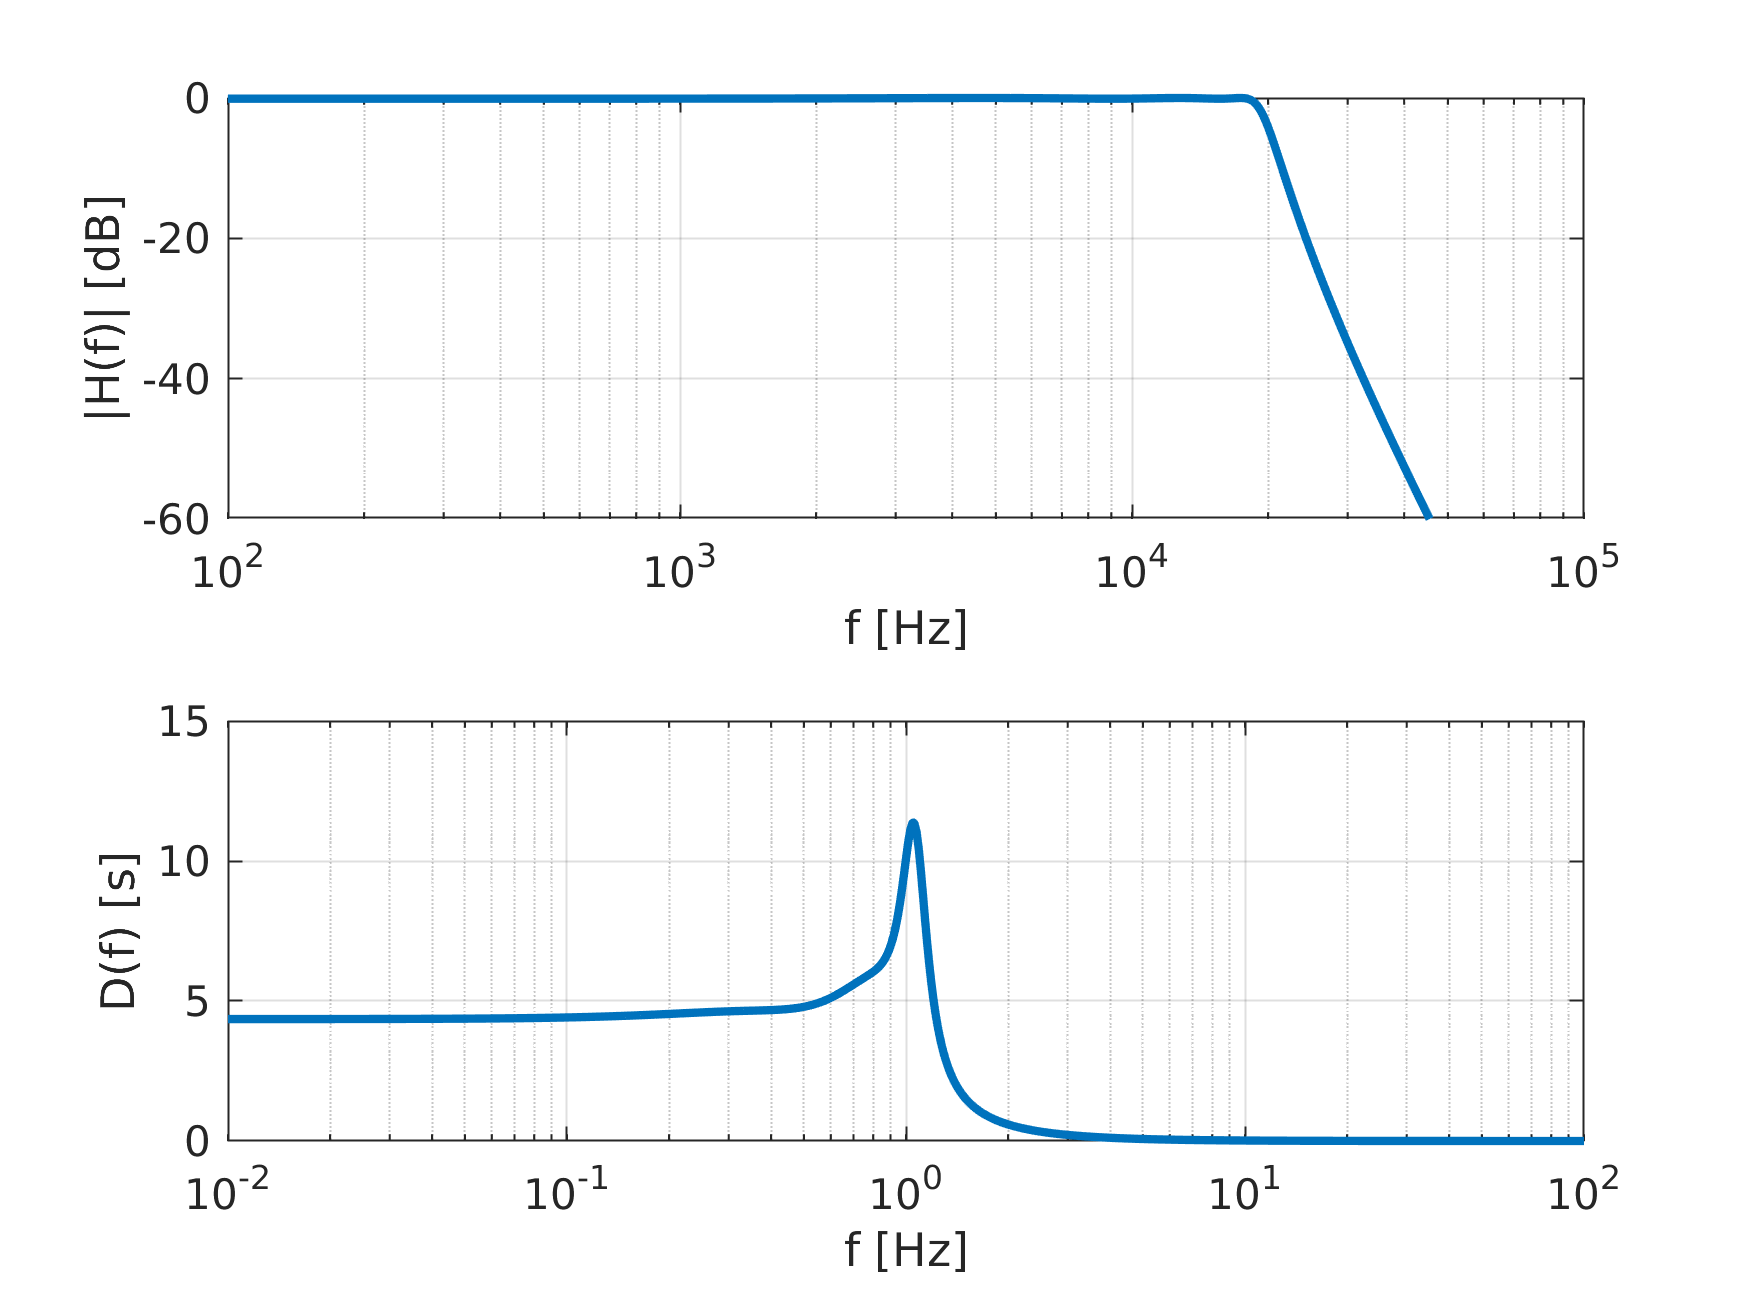
\includegraphics[width=1\textwidth]{matlab/filter_cheb1_denorm.png}
	\caption{Denormeret 6.ordens filter karakteristik og guppeløbstid af Chebychev Type I ($0,1 \si{\decibel}$}
	\label{fig:filter_cheb1_denorm}
\end{figure}
\jj{ret matlab fil med denormineret grpdelay}

Det valgte filter vil således have en dæmpning ved foldningsfrekvensen $f_s/2 = 22,05 \si{\kilo\hertz}$ på
\jj{Beregning for filter dæmpning her.}	 

%\note{Gennemgang af fordele/ulæmper ved filter typerne}
%\note{endelig valg og begrundelse}

\subsection{Forventet aliasing ved valgte filter type}


\note{Beregninger og argumentation for SNR}

\section{Specifikation og dimensionering}\label{sec:filter_spec}
\note{sprecifikation som bi-quad systemer}
\note{hvor tæt ligger de beregnede komponent værdier i hold til de anvendte tabelværdier ?}
\note{Sallen Kay - metode 4 i afs matr.}
\note{Hvordan kommer aliasing til at have indflydelse på det endelige signal ved valg af 6. ordens filter} 


\section{Design og implementering}\label{sec:filter_design}
\note{Fremstilling i bi-quad print}
\note{Argumenteret valg er OpAmp -> den bedste der var som SMD}
\note{Kort begrundelse for enkelt R i metoden og brug af op til 4 stk. C som proto type -> hvordan ville det se ud hvis kun brugte den nærmeste C i serien og hvor stor indflydelse vil det have. Måske Sensitivitesmetoden eller H(jw) -> var det er klogt valg og måske lidt overdrevet.}

\section{Rekonstruktions filter}
\note{Hvorfor anvendes et tilsvarende AA filter på udgangen - lidt teori her}

